% $Id: evaluation.tex 1784 2012-04-27 23:29:31Z nicolas.cardozo $
% !TEX root = main.tex

\chapter{Evaluation}
\label{cha:evaluation}

To evaluate and validate this tool as a framework for the quality development 
of \ac{RL} programs, an initial empirical test is proposed with different test scenarios 
that may arise in the development of \ac{RL} programs. These scenarios range from 
the creation of an \ac{RL} program from scratch to the process of optimizing 
learning parameters, aiming to determine the specific values to start with 
to achieve the most optimal convergence for the program. The idea for each of these 
programs is to intentionally add a logic bug on it, which means that the code runs 
normally, but the expected output does not match the real output of the program. 
This was made by the intention of trying to see if this tool could actually improve the 
performance and development of \ac{RL} programs.

Subsequently, an evaluation of the tool is proposed with a group of students 
from the \ac{RL} course at the University of the Andes, in order to obtain 
feedback on the utility of the tool and potential improvements that can be made, 
and the utility in general of back in time debuggers for debugging \ac{RL} programs.
The evaluation guide made to the students is presented in \fref{sec:eval-guide}, in which 
is describe the purpose of the tool, the description of the activity with the steps on how to run and 
use the tool, a small documentation of the tool, and an small example.

Let's dive into the three exercises proposed for the evaluation of the tool. 

\section{Exercise 1: GridWorld}

The gridworld environment consists of a $n\times n$ ($10\times 10$ in our example) rectangular 
board/grid, in which each tile $(i,j)$ represents a specific state of the board. Tiles in the board may be 
walls, which agents cannot cross. Additionally, there are special exit 
tiles that give a positive or negative reward to agents, as shown in \fref{fig:gridworld}. All tile types 
are unknown to the agent that moves from a given starting point in the board, searching for the goal 
state (\ie exit states with positive reward of $1$). The agent moves from state to state, avoiding 
obstacles and incorrect exit states (which give a reward of $-1$ when used to exit). 

\begin{figure}[h]
  \centering
  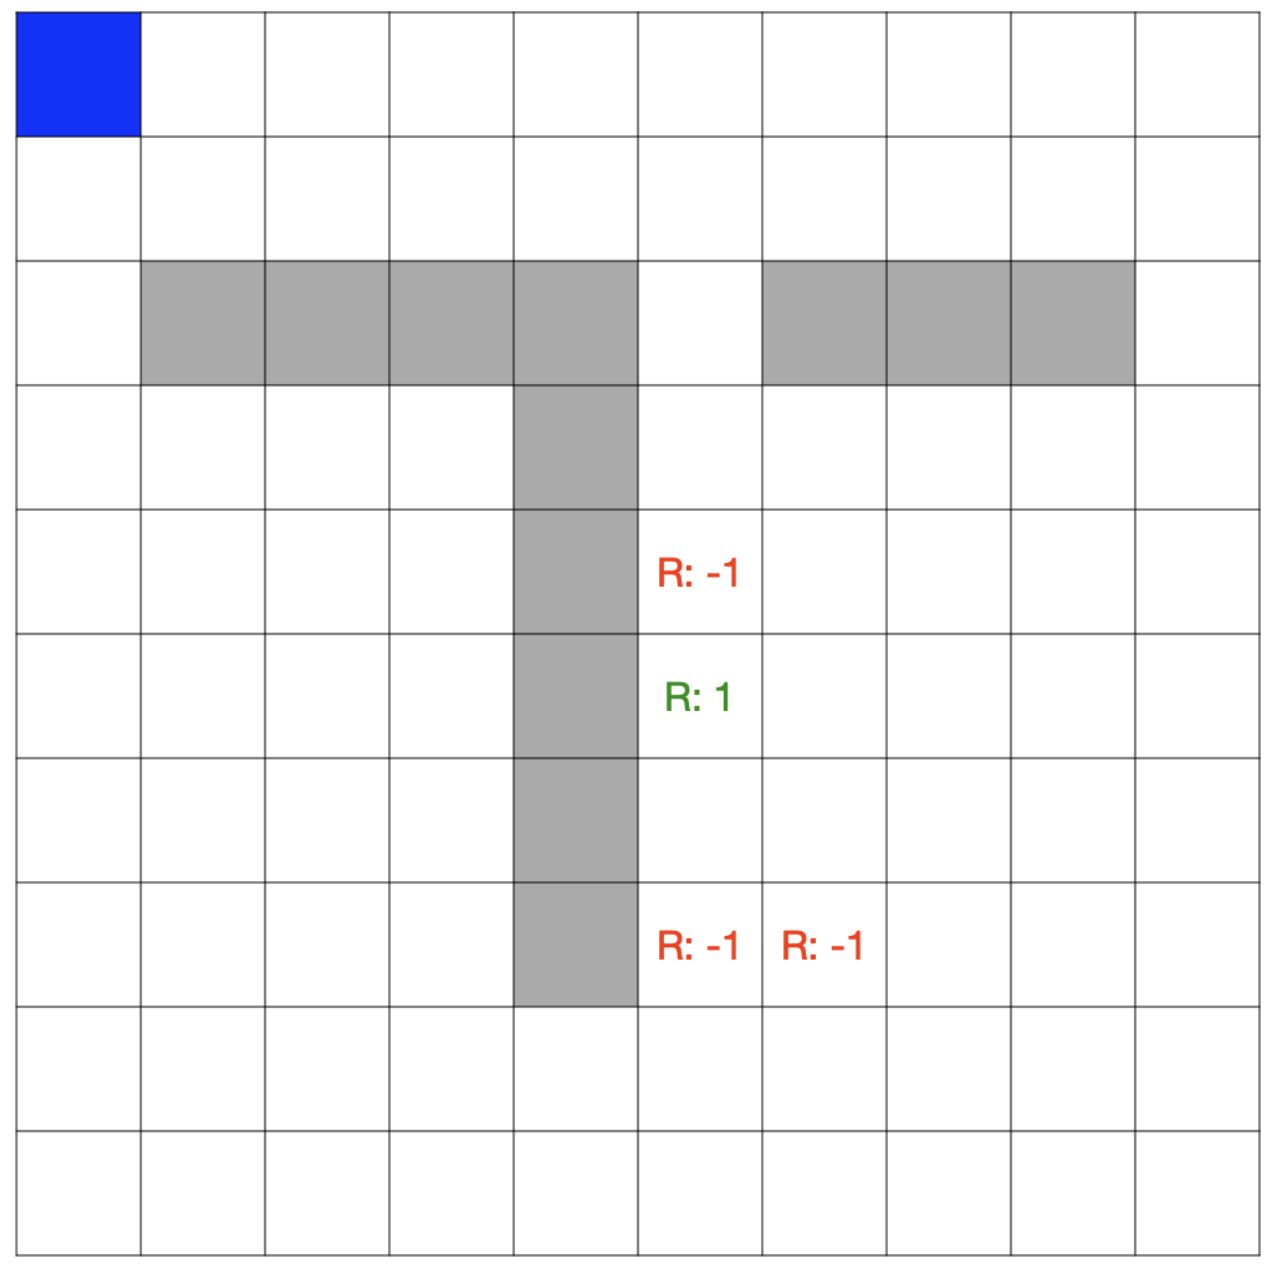
\includegraphics[width=0.5\columnwidth]{figures/gridworld.png}
  \caption{10x10 gridworld environment example}
  \label{fig:gridworld}
\end{figure}

Now, the idea of this example is to introduce the bug on $\epsilon$, which is the one that determines the 
probability of the action that must be taken next. This will introduce a wrong behavior for the \ac{RL} 
agent because $\epsilon$ will be so small that only in the first iteration the action will be taken randomly 
and in the follow interations the probability will be so small to take another action that the agent will not explore
other action policies. This is very bad specially for training purposes as we are supposed to have a very big 
probability to choose other actions and explore the grid. The idea in this task is that the students use 
Flik debugger to navigate throught the code and find out why is the agent not learning properly. And came 
with the solution of changing the value of $\epsilon$. 

\section{Exercise 2: Rooms}

The four rooms maze environment consists of a $13\times 13$ board/grid divided in $4$ sections 
(\ie rooms), with walls between them, and a door opening to go from one room to another, as shown 
in \fref{fig:rooms}. The agent's objective in this environment is to exit through the upper-left room 
(the green square) in the fewest possible steps. Reaching the exit state gives a reward of $1$, and no 
other action give a reward to the agent. In each episode the agent starts from any valid position in the 
grid, \eg the yellow square in the bottom-right room in the figure. 

\begin{figure}[h]
  \centering
  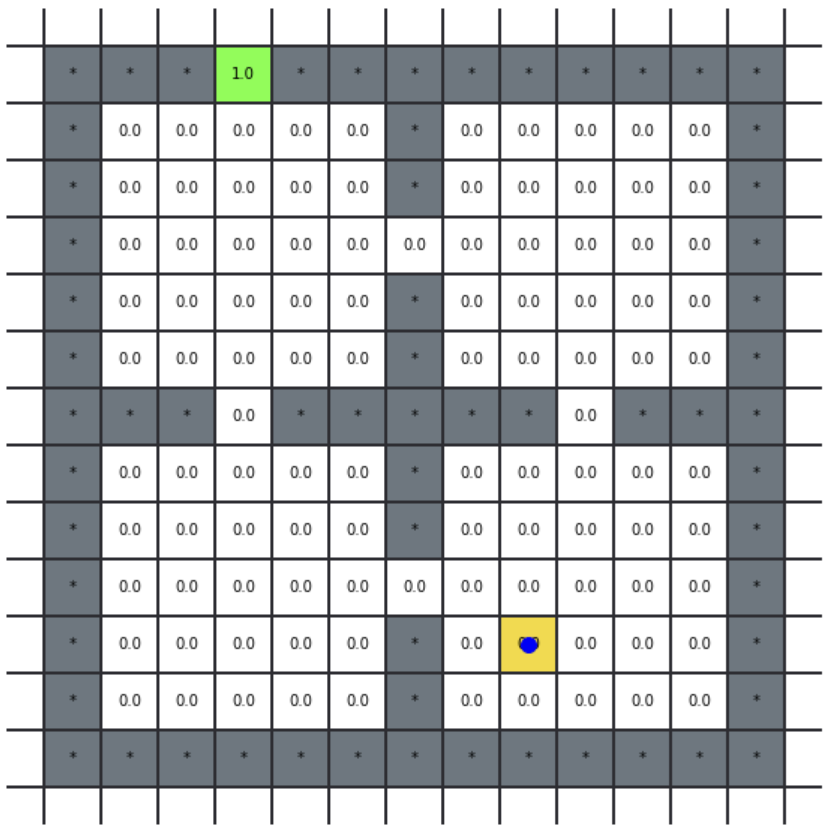
\includegraphics[width=0.5\columnwidth]{figures/rooms.png}
  \caption{Rooms environment example with associated rewards in each state}
  \label{fig:rooms}
\end{figure}

Now the idea of this example is to introduce the bug in the learning rate $\alpha$, on the QLearning equation 
so the original values for the learning rate alpha are exchanged like:

Original equation:
$
Q(s, a) \leftarrow (1-\alpha) Q(s, a) + \alpha \left( r + \gamma \max_{a'} Q(s', a') \right)
$

Wrong equation to debug:
$
Q(s, a) \leftarrow  \alpha Q(s, a) + (1-\alpha) \left( r + \gamma \max_{a'} Q(s', a') \right)
$

In the original equation,  $(1-\alpha) Q(s, a)$ is the current value and $\gamma \max_{a'} Q(s', a')$ the maximum 
reward that can be obtained from state $s'$. This means that if the learning rate is very small the current value 
will keep almost the same, turning a little bit towars the reward and the maximum value given the action, this will 
make that the agent learns by little steps towards the optimal policy. Now, in Q-learning, the learning rate $\alpha$
defines how much the old estimate $Q(s,a)$ is "revised" based on the new information. It ensures that over time, 
the algorithm balances past knowledge with current learning, gradually incorporating new information while 
retaining important aspects of previous learning. Changing the equation in this way will disrupt this balance. Specifically,
 $(1-\alpha)$ scales the difference between the new estimate and the old estimate. This makes the new information less influential as $\alpha$ gets larger, while the old value gets rescaled by $\alpha$, which doesn't align with the expected behavior of a Q-learning update. The idea in this task is that the students use Flik debugger to navigate throught 
the code and find out why is the agent not learning properly, and why is this happening. And came with the solution of changing the QLearning equation.

\section{Exercise 3: Cars}
In this example the agent is basically learning how to drive. The idea of this task is that the agent goes as 
fast as possible on the road without crashing with any other car. In the road there are only two lanes, and there 
are other cars that the agent must pass without crashing on them. The possible actions for the agent are: 
straight, slow\_down, speed\_up, steer\_left, steer\_right. The following is the visual interface of this environment.

\begin{figure}[h]
    \centering
    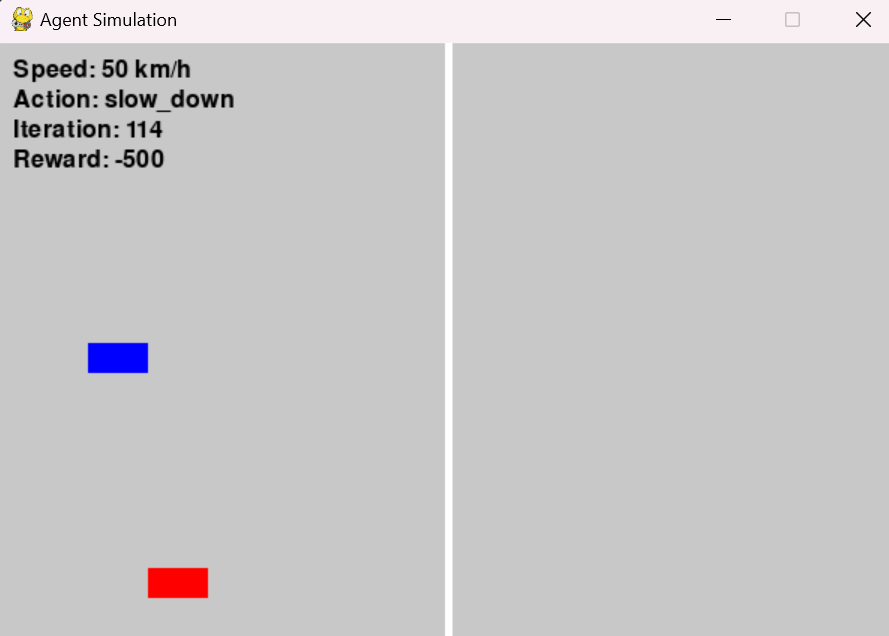
\includegraphics[width=0.5\textwidth]{figures/cars_example.png}
    \caption{Cars code example}
    \label{fig:cars-code-example}
\end{figure}

This is the largest excersice for the students to play with Flik and see why the agent was not learning. The main 
idea here was to modify the rewards so the agent weren't able to learn properly to go at the maximum velocity allowed.
The policy learned by the agent was to stop completely or go super slow, without learning how to drive. So the idea 
is that the students use Flik to come up with a solution for changing the rewards and make the agent learn a propper 
way how to drive at the maximum velocity, without stopping, and without crashing with other cars.

% Add way of evaluation, explanation about the survey, questions.
\section{Evaluation setup}
\label{sec:evaluation}
We invited 30 graduate students from Universidad de los Andes that attend the masters \ac{RL} course. Their 
responses were taken using a forms, and were anonymized and are avaible at \href{https://uniandes-my.sharepoint.com/:x:/g/personal/la_rodriguez_uniandes_edu_co/ESDy89Q-PgVBpYHEZ_CDh_IBhjhS35VFqNrlEjVw_ShY1w?e=lm319K}{this link}. 
The survey done is similar by the one done by the back in time debugger for JavaScript\cite{delorean23}. Also, the
questions are divided by 3 main sections:
\begin{itemize}
\item General knowledge questions: in which the student describes the familiarity they have using Python as a
programming language and their own experience using debuggers.
\item Task questions: in which each students describes the bug encountered in each of the tasks, and the solution 
 to the problem.
\item Feedback for the debugger usability: in which the student provides feedback about the use of the debugger 
for the tasks.
\end{itemize}



\endinput

